\documentclass[prb,12pt]{revtex4-2}

\usepackage{amsmath, amssymb,physics,amsfonts,amsthm}
\usepackage[most]{tcolorbox}
\usepackage{enumitem}
\usepackage{cancel}
\usepackage{booktabs}
\usepackage{polynom}
\usepackage{tikz}
\usepackage{hyperref}
\usepackage{enumitem}
\usepackage{transparent}
\usepackage{float}
\usepackage{multirow}
\newtheorem{Theorem}{Theorem}
\newtheorem{Proposition}{Theorem}
\newtheorem{Lemma}[Theorem]{Lemma}
\newtheorem{Corollary}[Theorem]{Corollary}
\newtheorem{Example}[Theorem]{Example}
\newtheorem{Remark}[Theorem]{Remark}
\theoremstyle{definition}
\newtheorem{Problem}{Problem}
\theoremstyle{definition}
\newtheorem{Definition}[Theorem]{Definition}
\newenvironment{parts}{\begin{enumerate}[label=(\alph*)]}{\end{enumerate}}
%tikz
\usetikzlibrary{patterns}
\usetikzlibrary{matrix}
%tcolorbox
\tcbset{breakable=true,toprule at break = 0mm,bottomrule at break = 0mm}
% definitions of number sets
\newcommand{\N}{\mathbb{N}}
\newcommand{\R}{\mathbb{R}}
\newcommand{\Z}{\mathbb{Z}}
\newcommand{\Q}{\mathbb{Q}}
\newcommand{\C}{\mathbb{C}}
\allowdisplaybreaks
\begin{document}
	\title{Lineare Algebra 2 Hausaufgabenblatt Nr. 12}
	\author{Jun Wei Tan}
	\email{jun-wei.tan@stud-mail.uni-wuerzburg.de}
	\affiliation{Julius-Maximilians-Universit\"{a}t W\"{u}rzburg}
	\date{\today}
	\maketitle

\section{Grund der Annahme}
\begin{tcolorbox}
	Weshalb könnte man mit den gegebenen Informationen davon ausgehen, dass die registrierten $\gamma$-Quanten einer Poissonverteilung folgen?
\end{tcolorbox}
Die Population ist unendlich. Die Anzahl von Versuche (hier: 336) ist groß. Die Größe $n\cdot p$ beträgt
\[\frac 12 \cdot 1\text{ s}\cdot \frac{1}{10\text{ years}}<9,\]
also die beste Verteilung ist eine Poissonverteilung.
\section{Datentabelle}
\begin{align*}
	\text{Mittelwert}:&~\mu=2,73214\\
	\text{Standardabweichung}:&~\sigma=1,67784
\end{align*}
\begin{table}[h]
	{\scriptsize
\begin{tabular}{cccccccccc}
	\toprule
	\textbf{Ereignisse} & 0 & 1 & 2 & 3 & 4 & 5 & 6 & 7 & 8 \\\midrule
	H\"{a}ufigkeit & 11 & 89 & 65 & 71 & 48 & 28 & 16 & 6 & 2 \\\midrule
	Relative H\"{a}ufigkeit & 0,032738 & 0,26488 & 0,19345 & 0,21131 & 0,14286 & 0,083333 & 0,047619 & 0,017857 & 0,0059524 \\\midrule
	Poisson-Wahrscheinlichkeit & 0,0650797 & 0,177807 & 0,242897 & 0,22121 & 0,151094 & 0,0825622 & 0,0375953 & 0,0146737 & 0,00501132 \\\bottomrule
\end{tabular}
}
\end{table}

\section{Histogramm}
\begin{figure}[h]
	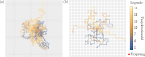
\includegraphics[width=0.6\textwidth]{fig1.pdf}
	\caption{}
\end{figure}

\section{Zentrale $\chi^2$ Verteilung}
Dichtefunktion:
\[f_{\chi^2_n}=\frac{1}{2^{\frac n2}\left(\frac n2-1\right)!}x^{\frac n2 - 1}\exp\left(-\frac x2\right)\]
\end{document}
